\subsection{Major Documentation Deliverables}

\subsubsection{Project Charter}
The initial version of the Project Charter is the goal of the first sprint and will be delivered on October 1st 2019. 
The Charter is expected to be updated mostly near the beginning of the project as the system requirements are finalized. Once this has been completed, items within the Charter will be checked after every sprint and any necessary updates will be added to the project backlog. The final version will be delivered at the end of the next semester, at the end of the project.

\subsubsection{System Requirements Specification}
The System Requirements Specification will be the goal of the second sprint and is expected to be delivered on the week of the 21st of October 2019. As we begin implementation, new requirements may become apparent or the feasability of previous requirements may come into question. As design decisions are made to address these issues, the System Requirements Specification will be updated to reflectthem.

\subsubsection{Architectural Design Specification}
The Architectural Design Specification will be the goal of the third sprint and is expected to be delivered on the week of the 11th of November 2019. As new design decisions are made, the Architectural Design Specification will be updated.

\subsubsection{Detailed Design Specification}
The Detailed Design Specification will be constantly looked at during the sprints and updated as implementation progresses. The final version is expected to be delivered at the end of the second semester.

\subsection{Recurring Sprint Items}

\subsubsection{Product Backlog}
System requirements will be broken up into discrete, manageable tasks that a single team member or pair of team members can address during a single sprint. These tasks will then be added to the Product Backlog. The Product Owner will prioritize the backlog and the Scrum master will assign the duties to individual members based on interests, skills, and which team they are participating in (hardware or software). The backlog will be stored and maintained in a GitHub Project page.

\subsubsection{Sprint Planning}
There will be eight sprints to be planned out by the Scrum Master in conjunction with the Product Owner.

\subsubsection{Sprint Goal}
The sprint goals will be decided by a team vote at a meeting prior to a sprint.

\subsubsection{Sprint Backlog}
The Product Owned will decide which items within the Product Backlog will be moved to the Sprint Backlog.

\subsubsection{Task Breakdown}
The Scrum Master and Product Owner will decide who is assigned which tasks. The decisions will be made based on interests, skills, and which team the member is a part of. Each team member will be responsible for maintaining their estimates for each of the tasks they are working on. 

\subsubsection{Sprint Burn Down Charts}
Time spent on tasks will be self reported by the team members and a burn down chart will be generated by the scrum master.

\begin{figure}[h!]
    \centering
    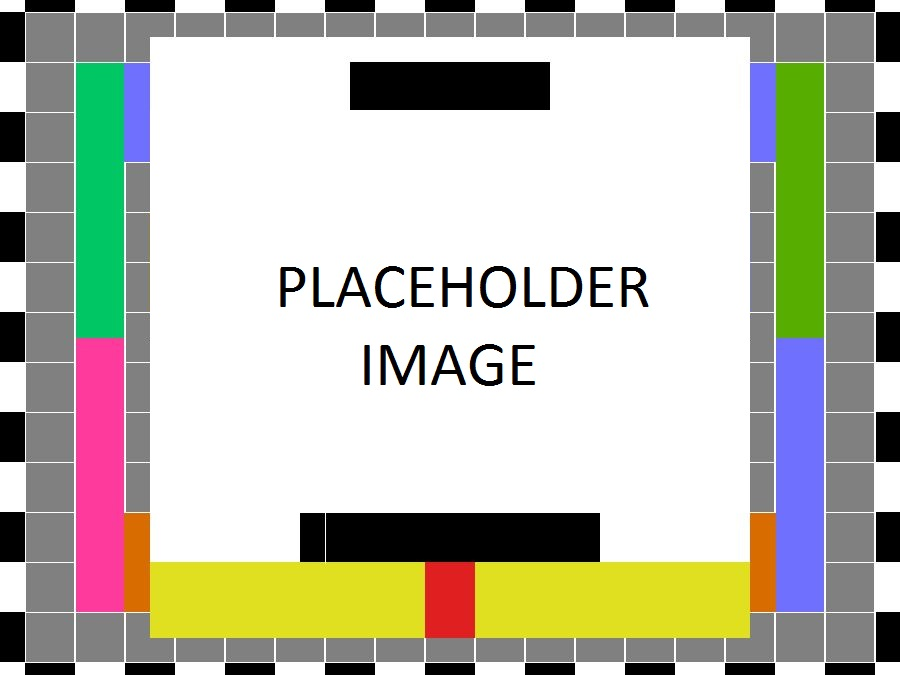
\includegraphics[width=0.5\textwidth]{images/test_image}
    \caption{Example sprint burn down chart}
\end{figure}

\subsubsection{Sprint Retrospective}
The Sprint Retrospective will take place immediately after a sprint and before the next sprint is planned. This will be an opportunity to raise any problems that members may have encoutered thoughout the sprint.

\subsubsection{Individual Status Reports}
Individual status reports will include a list of tasks a member is working on and their progress for each. Each member will be responsible for keeping their reports up to date.

\subsubsection{Engineering Notebooks}
The engineering notebooks will be signed periodically during stand-ups. Anyone within the team with knowledge of what is on a given notebook will be able to sign the notebook as a witness.

\subsection{Closeout Materials}

\subsubsection{System Prototype}
Our final System Prototype will be tested by someone who knows how to play a musical instrument for a final demonstration for the class.

\subsubsection{Project Poster}
The Project Poster will be depict the process we underwent to create the final product and include a depiction of the final prototype.

\subsubsection{Web Page}
Our project will have an informational webpage that will include links to the source code and the demo video.

\subsubsection{Demo Video}
The demo video will show a demonstration of the laser instrument being played as well as a step-by-step guide of how to configure it using the mobile app.

\subsubsection{Source Code}
The source code will be maintained on a GitHub repository. The resulting application code and schematics will be made available to the public under the GNU General Public License.

\subsubsection{Source Code Documentation}
Doxygen will be used to generate the source code documentation which will be published on the project web page.

\subsubsection{Hardware Schematics}
Hardware Schematics for the laser devices and the sound producing device will be made available throught the project web page.

\subsubsection{User Manual}
A user manual and set up video will be made available through the project web page.
